\documentclass[a4paper]{article}
\usepackage{geometry}
\usepackage{graphicx}
\usepackage{natbib}
\usepackage{amsmath}
\usepackage{amssymb}
\usepackage{amsthm}
\usepackage{paralist}
\usepackage{epstopdf}
\usepackage{tabularx}
\usepackage{longtable}
\usepackage{multirow}
\usepackage{multicol}
\usepackage[hidelinks]{hyperref}
\usepackage{fancyvrb}
\usepackage{algorithm}
\usepackage{algorithmic}
\usepackage{float}
\usepackage{paralist}
\usepackage[svgname]{xcolor}
\usepackage{enumerate}
\usepackage{array}
\usepackage{times}
\usepackage{url}
\usepackage{fancyhdr}
\usepackage{comment}
\usepackage{environ}
\usepackage{times}
\usepackage{textcomp}
\usepackage{caption}
\usepackage{bbm}


\urlstyle{rm}

\setlength\parindent{0pt} % Removes all indentation from paragraphs
\theoremstyle{definition}
\newtheorem{definition}{Definition}[]
\newtheorem{conjecture}{Conjecture}[]
\newtheorem{example}{Example}[]
\newtheorem{theorem}{Theorem}[]
\newtheorem{lemma}{Lemma}
\newtheorem{proposition}{Proposition}
\newtheorem{corollary}{Corollary}

\floatname{algorithm}{Procedure}
\renewcommand{\algorithmicrequire}{\textbf{Input:}}
\renewcommand{\algorithmicensure}{\textbf{Output:}}
\newcommand{\abs}[1]{\lvert#1\rvert}
\newcommand{\norm}[1]{\lVert#1\rVert}
\newcommand{\RR}{\mathbb{R}}
\newcommand{\CC}{\mathbb{C}}
\newcommand{\Nat}{\mathbb{N}}
\newcommand{\br}[1]{\{#1\}}
\DeclareMathOperator*{\argmin}{arg\,min}
\DeclareMathOperator*{\argmax}{arg\,max}
\renewcommand{\qedsymbol}{$\blacksquare$}

\definecolor{dkgreen}{rgb}{0,0.6,0}
\definecolor{gray}{rgb}{0.5,0.5,0.5}
\definecolor{mauve}{rgb}{0.58,0,0.82}

\newcommand{\Var}{\mathrm{Var}}
\newcommand{\Cov}{\mathrm{Cov}}

\newcommand{\vc}[1]{\boldsymbol{#1}}
\newcommand{\xv}{\vc{x}}
\newcommand{\Sigmav}{\vc{\Sigma}}
\newcommand{\alphav}{\vc{\alpha}}
\newcommand{\muv}{\vc{\mu}}

\newcommand{\red}[1]{\textcolor{red}{#1}}

\def\x{\mathbf x}
\def\y{\mathbf y}
\def\w{\mathbf w}
\def\v{\mathbf v}
\def\E{\mathbb E}
\def\V{\mathbb V}
\def\ind{\mathbbm 1}

% TO SHOW SOLUTIONS, include following (else comment out):
\newenvironment{soln}{
    \leavevmode\color{blue}\ignorespaces
}{}


\hypersetup{
%    colorlinks,
    linkcolor={red!50!black},
    citecolor={blue!50!black},
    urlcolor={blue!80!black}
}

\geometry{
  top=1in,            % <-- you want to adjust this
  inner=1in,
  outer=1in,
  bottom=1in,
  headheight=3em,       % <-- and this
  headsep=2em,          % <-- and this
  footskip=3em,
}


\pagestyle{fancyplain}
\lhead{\fancyplain{}{Homework 5}}
\rhead{\fancyplain{}{CS 760 Machine Learning}}
\cfoot{\thepage}

\title{\textsc{Homework 5}} % Title

%%% NOTE:  Replace 'NAME HERE' etc., and delete any "\red{}" wrappers (so it won't show up as red)

\author{
\red{$AKASH SHARMA$} \\
\red{$9081731771$}\\
} 

\date{}

\begin{document}

\maketitle 


\textbf{Instructions:} 
Although this is a programming homework, you only need to hand in a pdf answer file.
There is no need to submit the latex source or any code.
You can choose any programming language, as long as you implement the algorithm from scratch. 

Use this latex file as a template to develop your homework.
Submit your homework on time as a single pdf file to Canvas.
Please check Piazza for updates about the homework.



\section*{Linear Regression (100 pts total, 10 each)}

The Wisconsin State Climatology Office keeps a record on
the number of days Lake Mendota was covered by ice at
\url{http://www.aos.wisc.edu/~sco/lakes/Mendota-ice.html}.
Same for Lake Monona:
\url{http://www.aos.wisc.edu/~sco/lakes/Monona-ice.html}.
As with any real problems, the data is not as clean or as organized as one would like for machine learning.
Curate two clean data sets for each lake, respectively, starting from 1855-56 and ending in 2018-19.
Let $x$ be the year: for 1855-56, $x=1855$; for 2017-18, $x=2017$; and so on.
Let $y$ be the ice days in that year: for Mendota and 1855-56, $y=118$; for 2017-18, $y=94$; and so on.
Some years have multiple freeze thaw cycles such as 2001-02, that one should be $x=2001, y=21$.

\begin{enumerate}
\item
Plot year vs. ice days for the two lakes as two curves in the same plot.
Produce another plot for year vs. $y_{Monona} - y_{Mendota}$.

\begin{soln}
\begin{figure}[H]
	        \centering
	        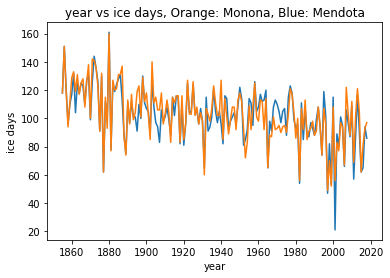
\includegraphics[width=0.4\textwidth]{1.png}
	    \end{figure}

\begin{figure}[H]
	        \centering
	        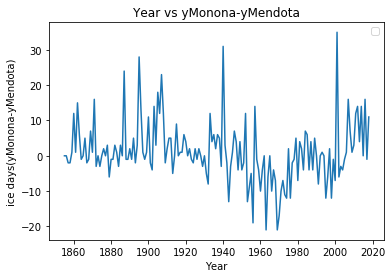
\includegraphics[width=0.4\textwidth]{2.png}
	    \end{figure}
\end{soln}


\item
Split the datasets: $x\le 1970$ as training, and $x>1970$ as test.
(Comment: due to the temporal nature this is NOT an iid split.  But we will work with it.)
On the training set, compute the sample mean $\bar y=\frac{1}{n}\sum_{i=1}^n y_i$ and the sample standard deviation $\sqrt{\frac{1}{n-1}\sum_{i=1}^n (y_i-\bar y)^2}$ for the two lakes, respectively.

\begin{soln}
Sample Mean (Mendota training set) = 107.18965517\\
Sample Standard Deviation (Mendota training set) = 16.74666159\\
Sample Mean (Monona training set) = 108.48275862\\
Sample Standard Deviation (Monona training set) = 18.12252154
\end{soln}

\item
Using training sets, train a linear regression model
$$\hat y_{Mendota} = \beta_0 + \beta_1 x + \beta_2 y_{Monona}$$
to predict $y_{Mendota}$.
Note: we are treating $y_{Monona}$ as an observed feature.
Do this by finding the closed-form MLE solution for $\beta=(\beta_0, \beta_1, \beta_2)^\top$ (no regularization):
$$\min_\beta {1\over n} \sum_{i=1}^n (x_i^\top \beta - y_i)^2.$$
Give the MLE formula in matrix form (define your matrices), then give the MLE value of $\beta_0, \beta_1, \beta_2$. 


\begin{soln}
We will take the derivative of $$\min_\beta {1\over n} \sum_{i=1}^n (x_i^\top \beta - y_i)^2.$$ with respect to $\beta$ and equate it to 0 to minimise the above.\\
$\Delta_\beta {1\over n} \sum_{i=1}^n (x_i^\top \beta - y_i)^2$\\
$ = \sum_{i=1}^{n}2(x_i^T \beta - y_i)x_i$\\
$ = 2 \sum_{i=1}^{n}(x_ix_i^T \beta - y_ix_i)$\\
Equating the above to 0, we get, \\
$\min_\beta = (\sum_{i=1}^{n}x_ix_i^T)^{-1}(\sum_{i=1}^{n}y_ix_i)$\\


$\hat y$ can also be written as $\hat y = X\beta$,\\
where X is the nxd matrix consisting of each training set $x_i$ for i in $[1...n]$ and $\beta$ is the column matrix\\
$\min_\beta \|X\beta - y\|^2$\\
To find the $\min_\beta$, we will take the derivative and equate it to 0, that is\\
$\Delta_\beta \|X\beta - y\|^2 = 2X^T(X\beta - y) $\\
$2X^T(X\beta - y) = 0$\\
$\min_\beta = (X^TX)^{-1}X^Ty$

MLE value for $\beta$ is, $[-64.18276629, 0.04122456, 0.85295063]^T$

\end{soln}



\item
Using the MLE above, give the (1) mean squared error and (2) $R^2$ values on the Mendota test set.
(You will need to use the Monona test data as observed features.)

\begin{soln}
The mean squared error is 124.26409484\\
$R^2$ values on Mendota test set is 0.71049007
\end{soln}


\item
``Reset'' to Q3, but this time use gradient descent to learn the $\beta$'s.
Recall our objective function is the mean squared error on the training set:
$${1\over n} \sum_{i=1}^n (x_i^\top \beta - y_i)^2.$$
Derive the gradient.

\begin{soln}
In gradient descent, $\beta_{t+1} = \beta_t - \eta_t \Delta_\beta f(\beta_t)$\\
where our objective function is $f(\beta_t) = {1\over n} \sum_{i=1}^n (x_i^\top \beta - y_i)^2$\\
Finding the derivative of $f(\beta_t)$ w.r.t $\beta$\\
$\Delta_\beta f(\beta_t) = {1\over n} \sum_{i=1}^{n}2(x_i^T\beta - y_i)\Delta_\beta(x_i^T\beta)$ $ = {1\over n} \sum_{i=1}^{n}2(x_i^T\beta - y_i)x_i$\\
$ \Delta_\beta f(\beta_t) = {2\over n} \sum_{i=1}^{n}(x_ix_i^T\beta - y_ix_i)$\\
Hence,\\
$\beta_{t+1} = \beta_t - \eta_t {2\over n} \sum_{i=1}^{n}(x_ix_i^T\beta - y_ix_i)$\\

\end{soln}

\item
Implement gradient descent.  Initialize $\beta_0= \beta_1= \beta_2=0$.  Use a fixed stepsize parameter $\eta=0.1$ and print the first 10 iteration's objective function value.
Tell us if further iterations make your gradient descent converge, and if yes when; compare the $\beta$'s to the closed-form solution.
Try other $\eta$ values and tell us what happens.
\textbf{Hint:} Update $\beta_0, \beta_1, \beta_2$ simultaneously in an iteration.  Don't use a new $\beta_0$ to calculate $\beta_1$, and so on.

\begin{soln}
	
Starting with $\beta = [0, 0, 0]^T$ and $\eta=0.1$, we get the below values: 

$\beta = [0, 0, 0]^T$\\
iteration1 objective function value: 11767.655172413793\\
\\
$\beta = [2.14379310e+01, 4.09649931e+04, 2.37904828e+03]^T$\\
iteration 2 objective function value: 6180350808297761.0\\
\\
$\beta = [-1.57206884e+07, -3.00748795e+10, -1.70345111e+09]^T$\\
iteration 3 objective function value: 3.330626781514361e+27\\
\\
$\beta = [1.15405879e+13, 2.20780301e+16, 1.25050392e+15]^T$\\
iteration 4 objective function value: 1.794894028506588e+39\\
\\
$\beta = [-8.47196890e+18, -1.62075266e+22, -9.17997455e+20]^T$\\
iteration 5 objective function value: 9.672787691041734e+50\\
\\
$\beta = [6.21928952e+24, 1.18979781e+28, 6.73903790e+26]^T$\\
iteration 6 objective function value: 5.212721209720436e+62\\
\\
$\beta = [-4.56559302e+30, -8.73432978e+33, -4.94714136e+32]^T$\\
iteration 7 objective function value: 2.809165597156089e+74\\
\\
$\beta = [3.35161108e+36, 6.41188917e+39, 3.63170649e+38]^T$\\
iteration 8 objective function value: 1.5138755814390735e+86\\
\\
$\beta = [-2.46042448e+42, -4.70698081e+45, -2.66604308e+44]^T$\\
iteration 9 objective function value: 8.158363032772645e+97\\
\\
$\beta = [1.80620259e+48, 3.45540414e+51, 1.95714762e+50]^T$\\
iteration 10 objective function value: 4.396589005765003e+109\\
\\


The $\beta$ values for the closed form solution are:  $[-64.18276629, 0.04122456, 0.85295063]^T$\\

On decreasing the value of $\eta$, the objective function does not converge (for $\eta$ = 0.1 , 0.001, 0.0001, 0.00001, 0.000001, 0.000001), it actually diverges. Decreasing the value of $eta$ beyond $10^{-7}$, and number of iterations greater than or equal to 60000, converges the objective function.
	
\end{soln}

\item
As preprocessing, normalize your year and Monona features (but not $y_{Mendota}$).
Then repeat Q6.

\begin{soln}

After normalizing the data, we get the following values:

$\beta = [0,0,0]^T$\\
iteration 1 objective function value: 11767.655172413793\\
\\
$\beta = [21.43793103, -1.04221356,  2.94674105]^T$\\
iteration 2 objective function value:  7545.998373501811\\
\\
$\beta = [38.58827586, -1.62669734,  5.22041022]^T$\\
iteration 3 objective function value:  4850.273518530398\\
\\
$\beta = [52.30855172, -1.90155878,  6.99346337]^T$\\
iteration 4 objective function value:  3127.473895121937\\
\\
$\beta = [63.28477241, -1.97084467,  8.39154266]^T$\\
iteration 5 objective function value:  2025.60791967957\\
\\
$\beta = [72.06574897, -1.90726621,  9.5065129 ]^T$\\
iteration 6 objective function value:  1320.3620154290259\\
\\
$\beta = [79.09053021, -1.76129017, 10.40582881]^T$\\
iteration 7 objective function value:  868.6443341670561\\
\\
$\beta = [84.7103552,  -1.56762933, 11.13927032]^T$\\
iteration 8 objective function value:  579.097480654567\\
\\
$\beta = [89.20621519, -1.34987216, 11.7437894 ]^T$\\
iteration 9 objective function value:  393.3511885316238\\
\\
$\beta = [92.80290319, -1.1237815,  12.24700146]^T$\\
iteration 10 objective function value:  274.0870881867739\\

On decreasing the value of $\eta$, the objective function converges slowly (convergence rate decreases).
\\For $\eta = 0.1$, objective function starts converging from 26th iteration.
\\for $\eta = 0.01$, objective function starts converging from 264th iteration.

The value of $\beta$ obtained in close-form solution is lesser than the one obtained above.

The minimum value of objective function is 57.87255167863114. Value of $\beta$ at minimum objective function value = $[106.7847041,0.968649,15.03648842]^T$. 

\end{soln}


\item 
``Reset'' to Q3 (no normalization,  use closed-form solution), but train a linear regression model without using Monona:
$$\hat y_{Mendota} = \gamma_0 + \gamma_1 x.$$
  \begin{enumerate}
  \item Interpret the sign of $\gamma_1$.

  \begin{soln}
  $\gamma = [ 4.06111060e+02,-1.56298774e-01]^T$
  \\Here, since, the sign of $\gamma_1$ is negative, so, as the value of x (year) increases, $\hat y_{Mendota}$ decreases.
  \end{soln}

  \item Some analysts claim that because $\beta_1$ the closed-form solution in Q3 is positive, fixing all other factors, as the years go by the number of Mendota ice days will increase, namely the model in Q3 indicates a cooling trend. Discuss this viewpoint, relate it to question 8(a).
 \begin{soln}
\\The value of $\hat y_{Mendota}$ is dependent on both the the year (x) and the $y_{Monona}$. So, even if $\beta_1$ is positive in the closed form solution, we cannot say that $\hat y_{Mendota}$ increases as x increases. In 8(a), the  $\hat y_{Mendota}$ is dependent only on the value of year (x), and as the value of $\gamma_1$ is negative above, we can say that as x (year) increases, $\hat y_{Mendota}$ decreases.

 \end{soln}

  \end{enumerate}

\item
Of course, Weka has linear regression.  Reset to Q3.  Save the training data in .arff format for Weka.  Use classifiers / functions / LinearRegression.  Choose ``Use training set.''  
  Bring up Linear Regression options, set ``ridge'' to 0 so it does not regularize.  Run it and tell us the model: it is in the output in the form of ``$\beta_1$ * year + $\beta_2$ * Monona + $\beta_0$.'' 


\begin{soln}
y = 0.0412 * year + 0.853  * Monona +  -64.1828
\end{soln}


\item Ridge regression.
\begin{enumerate}
\item
Then set ridge to 1 and tell us the resulting Weka model.

\begin{soln}
y = 0.0387 * year + 0.8436 * Monona + -58.3961
\end{soln}


\item
Meanwhile, derive the closed-form solution in matrix form for the ridge regression problem:
$$\min_\beta \left({1\over n} \sum_{i=1}^n (x_i^\top \beta - y_i)^2 \right) + \lambda \|\beta\|_A^2$$
where 
$$\|\beta\|_A^2 := \beta^\top A \beta$$
and
$$A=
\begin{bmatrix}
0 & 0 & 0 \\
0 & 1 & 0 \\
0 & 0 & 1
\end{bmatrix}.$$
This $A$ matrix has the effect of NOT regularizing the bias $\beta_0$, which is standard practice in ridge regression.
Note: Derive the closed-form solution, do not blindly copy lecture notes.

\begin{soln}
For Ridge Regression, the objective function, $$\min_\beta \left({1\over n} \sum_{i=1}^n (x_i^\top \beta - y_i)^2 \right) + \lambda \|\beta\|_A^2$$\\
Since, we are given, $\|\beta\|_A^2 := \beta^\top A \beta$, simplifying further,

$\beta^\top A \beta = [\beta_0,\beta_1,\beta_2]
\begin{bmatrix}
0 & 0 & 0 \\
0 & 1 & 0 \\
0 & 0 & 1
\end{bmatrix}
\begin{bmatrix}
\beta_0\\
\beta_1\\
\beta_2
\end{bmatrix}
$

$ = \beta_1^2 + \beta_2^2$\\

Putting the above value in the objective function, we get,\\
$$
\min_\beta \left({1\over n} \sum_{i=1}^n (x_i^\top \beta - y_i)^2 \right) + \lambda(\beta_1^2 + \beta_2^2)
$$\\

To get $\min_\beta$, we will find the derivative of the above function w.r.t $\beta$, and equate that to 0.\\

On differentiating, and equating to 0, we get \\
${2\over n}(2X^TX\beta - 2X^Ty) + \lambda[0,2\beta_1,2\beta_2] $
$ = {2\over n}(2X^TX\beta - 2X^Ty) + 2\lambda A\beta = 0$\\

$(X^TX\beta - 2X^Ty) + 2n\lambda A\beta = 0$\\
$(X^TX+2n\lambda A)\beta - 2X^Ty = 0$
\\Therefore,
$\min_\beta = (X^TX+n\lambda A)^{-1}X^Ty$

\end{soln}	





\item
Let $\lambda=1$ and tell us the value of $\beta$ from your ridge regression model.


\begin{soln}
Substituting the value of $\lambda=1$, we get, $\beta$ =\\
$[-62.32947227729614, 0.04043908716837768, 0.8497145022134832]$\\
\end{soln}



\end{enumerate}

\end{enumerate}

\end{document}
\bibliographystyle{apalike}
\end{document}
